% Options for packages loaded elsewhere
% Options for packages loaded elsewhere
\PassOptionsToPackage{unicode}{hyperref}
\PassOptionsToPackage{hyphens}{url}
%
\documentclass[
  ignorenonframetext,
  aspectratio=169,
  russian,
]{beamer}
\newif\ifbibliography
\usepackage{pgfpages}
\setbeamertemplate{caption}[numbered]
\setbeamertemplate{caption label separator}{: }
\setbeamercolor{caption name}{fg=normal text.fg}
\beamertemplatenavigationsymbolshorizontal
% remove section numbering
\setbeamertemplate{part page}{
  \centering
  \begin{beamercolorbox}[sep=16pt,center]{part title}
    \usebeamerfont{part title}\insertpart\par
  \end{beamercolorbox}
}
\setbeamertemplate{section page}{
  \centering
  \begin{beamercolorbox}[sep=12pt,center]{section title}
    \usebeamerfont{section title}\insertsection\par
  \end{beamercolorbox}
}
\setbeamertemplate{subsection page}{
  \centering
  \begin{beamercolorbox}[sep=8pt,center]{subsection title}
    \usebeamerfont{subsection title}\insertsubsection\par
  \end{beamercolorbox}
}
% Prevent slide breaks in the middle of a paragraph
\widowpenalties 1 10000
\raggedbottom
\AtBeginPart{
  \frame{\partpage}
}
\AtBeginSection{
  \ifbibliography
  \else
    \frame{\sectionpage}
  \fi
}
\AtBeginSubsection{
  \frame{\subsectionpage}
}
\usepackage{iftex}
\ifPDFTeX
  \usepackage[T1]{fontenc}
  \usepackage[utf8]{inputenc}
  \usepackage{textcomp} % provide euro and other symbols
\else % if luatex or xetex
  \usepackage{unicode-math} % this also loads fontspec
  \defaultfontfeatures{Scale=MatchLowercase}
  \defaultfontfeatures[\rmfamily]{Ligatures=TeX,Scale=1}
\fi
\usepackage{lmodern}

\ifPDFTeX\else
  % xetex/luatex font selection
\fi
% Use upquote if available, for straight quotes in verbatim environments
\IfFileExists{upquote.sty}{\usepackage{upquote}}{}
\IfFileExists{microtype.sty}{% use microtype if available
  \usepackage[]{microtype}
  \UseMicrotypeSet[protrusion]{basicmath} % disable protrusion for tt fonts
}{}


\usepackage{longtable,booktabs,array}
\usepackage{calc} % for calculating minipage widths
\usepackage{caption}
% Make caption package work with longtable
\makeatletter
\def\fnum@table{\tablename~\thetable}
\makeatother
\usepackage{graphicx}
\makeatletter
\newsavebox\pandoc@box
\newcommand*\pandocbounded[1]{% scales image to fit in text height/width
  \sbox\pandoc@box{#1}%
  \Gscale@div\@tempa{\textheight}{\dimexpr\ht\pandoc@box+\dp\pandoc@box\relax}%
  \Gscale@div\@tempb{\linewidth}{\wd\pandoc@box}%
  \ifdim\@tempb\p@<\@tempa\p@\let\@tempa\@tempb\fi% select the smaller of both
  \ifdim\@tempa\p@<\p@\scalebox{\@tempa}{\usebox\pandoc@box}%
  \else\usebox{\pandoc@box}%
  \fi%
}
% Set default figure placement to htbp
\def\fps@figure{htbp}
\makeatother



\ifLuaTeX
\usepackage[bidi=basic,provide=*]{babel}
\else
\usepackage[bidi=default,provide=*]{babel}
\fi
% get rid of language-specific shorthands (see #6817):
\let\LanguageShortHands\languageshorthands
\def\languageshorthands#1{}


\setlength{\emergencystretch}{3em} % prevent overfull lines

\providecommand{\tightlist}{%
  \setlength{\itemsep}{0pt}\setlength{\parskip}{0pt}}



 

\usepackage[]{csquotes}

\IfFileExists{plex-otf.sty}{
  %% Full TeXlive
  % \usepackage[%
  %   % math,
  %   RM={Scale=0.94},SS={Scale=0.94},SScon={Scale=0.94},TT={Scale=MatchLowercase,FakeStretch=0.9},DefaultFeatures={Ligatures=Common}
  % ]{plex-otf}
}{
  %% TinyTeX
  \usepackage{libertine}
}

%%% Load theme
% https://deic.uab.cat/~iblanes/beamer_gallery/
\IfFileExists{beamerthemegotham.sty}{
  %% Full TeXlive
  \usetheme{gotham}
  \gothamset{
    numbering=totalpagenumber,
    parttocframe default=off,
    sectiontocframe default=off,
    subsectiontocframe default=off,
  }
}{
  %% TinyTeX
  \usetheme{Madrid}
}
\makeatletter
\@ifpackageloaded{caption}{}{\usepackage{caption}}
\AtBeginDocument{%
\ifdefined\contentsname
  \renewcommand*\contentsname{Содержание}
\else
  \newcommand\contentsname{Содержание}
\fi
\ifdefined\listfigurename
  \renewcommand*\listfigurename{Список иллюстраций}
\else
  \newcommand\listfigurename{Список иллюстраций}
\fi
\ifdefined\listtablename
  \renewcommand*\listtablename{Список таблиц}
\else
  \newcommand\listtablename{Список таблиц}
\fi
\ifdefined\figurename
  \renewcommand*\figurename{Рисунок}
\else
  \newcommand\figurename{Рисунок}
\fi
\ifdefined\tablename
  \renewcommand*\tablename{Таблица}
\else
  \newcommand\tablename{Таблица}
\fi
}
\@ifpackageloaded{float}{}{\usepackage{float}}
\floatstyle{ruled}
\@ifundefined{c@chapter}{\newfloat{codelisting}{h}{lop}}{\newfloat{codelisting}{h}{lop}[chapter]}
\floatname{codelisting}{Список}
\newcommand*\listoflistings{\listof{codelisting}{Листинги}}
\makeatother
\makeatletter
\makeatother
\makeatletter
\@ifpackageloaded{caption}{}{\usepackage{caption}}
\@ifpackageloaded{subcaption}{}{\usepackage{subcaption}}
\makeatother

\usepackage{bookmark}
\IfFileExists{xurl.sty}{\usepackage{xurl}}{} % add URL line breaks if available
\urlstyle{same}
\hypersetup{
  pdftitle={Операционные системы},
  pdfauthor={Абу Зейтун Саед Фатхи Бадер},
  pdflang={ru-RU},
  hidelinks,
  pdfcreator={LaTeX via pandoc}}


\title{Операционные системы}
\subtitle{Командная оболочка Midnight Commander}
\author{Абу Зейтун Саед Фатхи Бадер}
\date{2026-03-24}

\begin{document}
\frame{\titlepage}

\renewcommand*\contentsname{Содержание}
\begin{frame}[allowframebreaks]
  \frametitle{Содержание}
  \setcounter{tocdepth}{1}
  \tableofcontents
\end{frame}
\setcounter{tocdepth}{1}
\tableofcontents
}

\section{Цели и задачи
работы}\label{ux446ux435ux43bux438-ux438-ux437ux430ux434ux430ux447ux438-ux440ux430ux431ux43eux442ux44b}

\begin{frame}{Цель лабораторной работы}
\phantomsection\label{ux446ux435ux43bux44c-ux43bux430ux431ux43eux440ux430ux442ux43eux440ux43dux43eux439-ux440ux430ux431ux43eux442ux44b}
Ознакомление с файловой системой Linux, её структурой, именами и
содержанием каталогов. Приобретение практических навыков по применению
команд для работы с файлами и каталогами, по управлению процессами, по
проверке использования диска и обслуживанию файловой системы.
\end{frame}

\begin{frame}{Задачи лабораторной работы}
\phantomsection\label{ux437ux430ux434ux430ux447ux438-ux43bux430ux431ux43eux440ux430ux442ux43eux440ux43dux43eux439-ux440ux430ux431ux43eux442ux44b}
1 Изучить возможности Midnight Commander

2 Изучить редактор Midnight Commander
\end{frame}

\section{Процесс выполнения лабораторной
работы}\label{ux43fux440ux43eux446ux435ux441ux441-ux432ux44bux43fux43eux43bux43dux435ux43dux438ux44f-ux43bux430ux431ux43eux440ux430ux442ux43eux440ux43dux43eux439-ux440ux430ux431ux43eux442ux44b}

\begin{frame}{Работа с Midnight Commander}
\phantomsection\label{ux440ux430ux431ux43eux442ux430-ux441-midnight-commander}
\begin{figure}

{\centering 
\includegraphics[width=0.7\linewidth,height=0.7\textheight]{image/01.png}

}

\caption{Запуск mc}

\end{figure}%
\end{frame}

\begin{frame}{Работа с Midnight Commander}
\phantomsection\label{ux440ux430ux431ux43eux442ux430-ux441-midnight-commander-1}
\begin{figure}

{\centering 
\includegraphics[width=0.7\linewidth,height=0.7\textheight]{image/02.png}

}

\caption{Выделение}

\end{figure}%
\end{frame}

\begin{frame}{Работа с Midnight Commander}
\phantomsection\label{ux440ux430ux431ux43eux442ux430-ux441-midnight-commander-2}
\begin{figure}

{\centering 
\includegraphics[width=0.7\linewidth,height=0.7\textheight]{image/03.png}

}

\caption{Отмена}

\end{figure}%
\end{frame}

\begin{frame}{Работа с Midnight Commander}
\phantomsection\label{ux440ux430ux431ux43eux442ux430-ux441-midnight-commander-3}
\begin{figure}

{\centering 
\includegraphics[width=0.7\linewidth,height=0.7\textheight]{image/04.png}

}

\caption{Копирование}

\end{figure}%
\end{frame}

\begin{frame}{Работа с Midnight Commander}
\phantomsection\label{ux440ux430ux431ux43eux442ux430-ux441-midnight-commander-4}
\begin{figure}

{\centering 
\includegraphics[width=0.7\linewidth,height=0.7\textheight]{image/05.png}

}

\caption{Перемещение}

\end{figure}%
\end{frame}

\begin{frame}{Работа с Midnight Commander}
\phantomsection\label{ux440ux430ux431ux43eux442ux430-ux441-midnight-commander-5}
\begin{figure}

{\centering 
\includegraphics[width=0.7\linewidth,height=0.7\textheight]{image/06.png}

}

\caption{Информация}

\end{figure}%
\end{frame}

\begin{frame}{Работа с Midnight Commander}
\phantomsection\label{ux440ux430ux431ux43eux442ux430-ux441-midnight-commander-6}
\begin{figure}

{\centering 
\includegraphics[width=0.7\linewidth,height=0.7\textheight]{image/07.png}

}

\caption{Быстрый просмотр}

\end{figure}%
\end{frame}

\begin{frame}{Работа с Midnight Commander}
\phantomsection\label{ux440ux430ux431ux43eux442ux430-ux441-midnight-commander-7}
\begin{figure}

{\centering 
\includegraphics[width=0.7\linewidth,height=0.7\textheight]{image/08.png}

}

\caption{Информация}

\end{figure}%
\end{frame}

\begin{frame}{Работа с Midnight Commander}
\phantomsection\label{ux440ux430ux431ux43eux442ux430-ux441-midnight-commander-8}
\begin{figure}

{\centering 
\includegraphics[width=0.7\linewidth,height=0.7\textheight]{image/09.png}

}

\caption{Дерево каталогов}

\end{figure}%
\end{frame}

\begin{frame}{Работа с Midnight Commander}
\phantomsection\label{ux440ux430ux431ux43eux442ux430-ux441-midnight-commander-9}
\begin{figure}

{\centering 
\includegraphics[width=0.7\linewidth,height=0.7\textheight]{image/10.png}

}

\caption{Просмотр содержимого текстового файла}

\end{figure}%
\end{frame}

\begin{frame}{Работа с Midnight Commander}
\phantomsection\label{ux440ux430ux431ux43eux442ux430-ux441-midnight-commander-10}
\begin{figure}

{\centering 
\includegraphics[width=0.7\linewidth,height=0.7\textheight]{image/11.png}

}

\caption{Отредактируем содержимое текстового файла без сохранения
результатов}

\end{figure}%
\end{frame}

\begin{frame}{Работа с Midnight Commander}
\phantomsection\label{ux440ux430ux431ux43eux442ux430-ux441-midnight-commander-11}
\begin{figure}

{\centering 
\includegraphics[width=0.7\linewidth,height=0.7\textheight]{image/12.png}

}

\caption{Создание каталога}

\end{figure}%
\end{frame}

\begin{frame}{Работа с Midnight Commander}
\phantomsection\label{ux440ux430ux431ux43eux442ux430-ux441-midnight-commander-12}
\begin{figure}

{\centering 
\includegraphics[width=0.7\linewidth,height=0.7\textheight]{image/13.png}

}

\caption{Копирование в файлов в созданный каталог}

\end{figure}%
\end{frame}

\begin{frame}{Работа с Midnight Commander}
\phantomsection\label{ux440ux430ux431ux43eux442ux430-ux441-midnight-commander-13}
\begin{figure}

{\centering 
\includegraphics[width=0.7\linewidth,height=0.7\textheight]{image/14.png}

}

\caption{Поиск файлов}

\end{figure}%
\end{frame}

\begin{frame}{Работа с Midnight Commander}
\phantomsection\label{ux440ux430ux431ux43eux442ux430-ux441-midnight-commander-14}
\begin{figure}

{\centering 
\includegraphics[width=0.7\linewidth,height=0.7\textheight]{image/15.png}

}

\caption{История команд}

\end{figure}%
\end{frame}

\begin{frame}{Работа с Midnight Commander}
\phantomsection\label{ux440ux430ux431ux43eux442ux430-ux441-midnight-commander-15}
\begin{figure}

{\centering 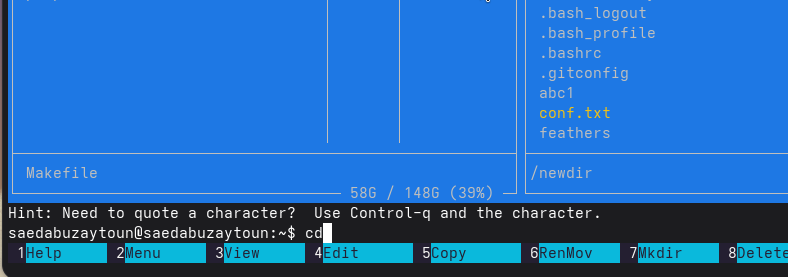
\includegraphics[width=0.7\linewidth,height=0.7\textheight]{image/16.png}

}

\caption{Переход в домашний каталог}

\end{figure}%
\end{frame}

\begin{frame}{Работа с Midnight Commander}
\phantomsection\label{ux440ux430ux431ux43eux442ux430-ux441-midnight-commander-16}
\begin{figure}

{\centering 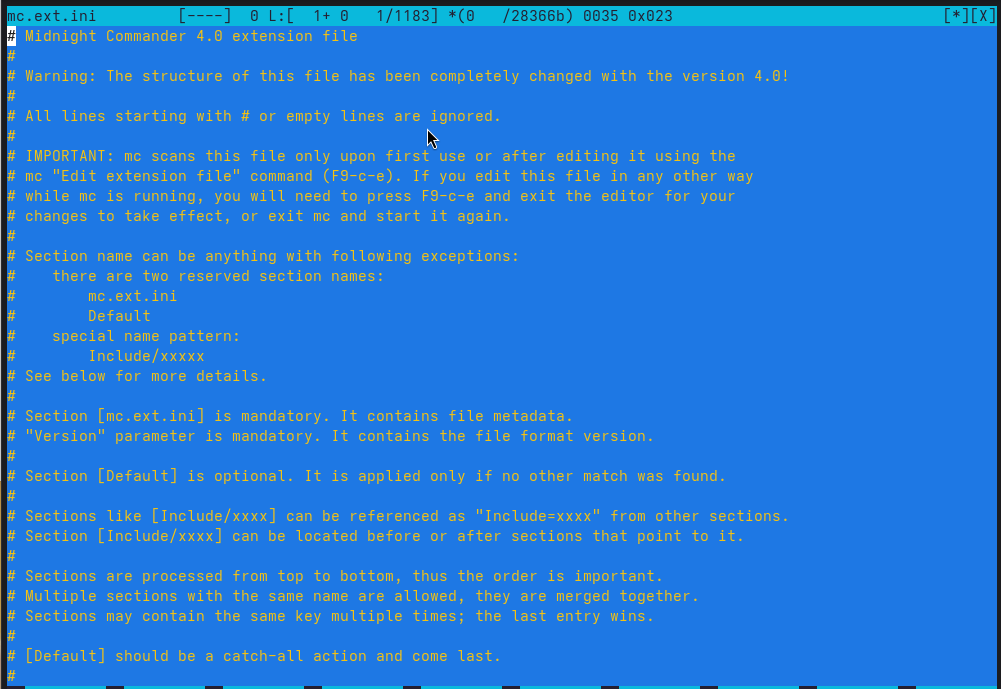
\includegraphics[width=0.7\linewidth,height=0.7\textheight]{image/17.png}

}

\caption{Просмотр файла расширений}

\end{figure}%
\end{frame}

\begin{frame}{Работа с Midnight Commander}
\phantomsection\label{ux440ux430ux431ux43eux442ux430-ux441-midnight-commander-17}
\begin{figure}

{\centering 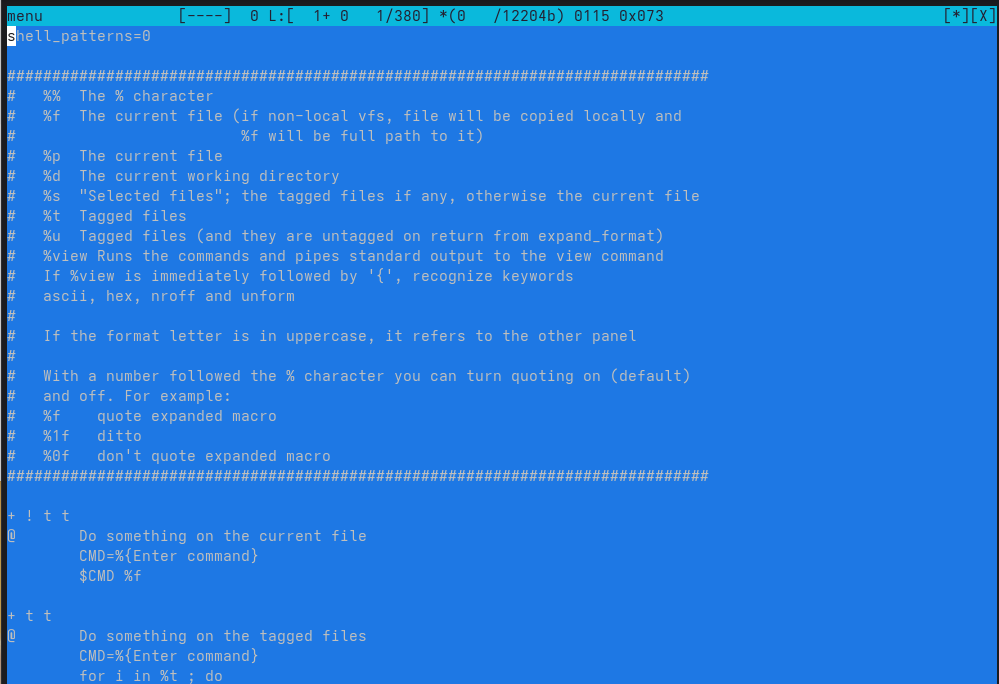
\includegraphics[width=0.7\linewidth,height=0.7\textheight]{image/18.png}

}

\caption{Просмотр файла меню}

\end{figure}%
\end{frame}

\begin{frame}{Работа с Midnight Commander}
\phantomsection\label{ux440ux430ux431ux43eux442ux430-ux441-midnight-commander-18}
\begin{figure}

{\centering 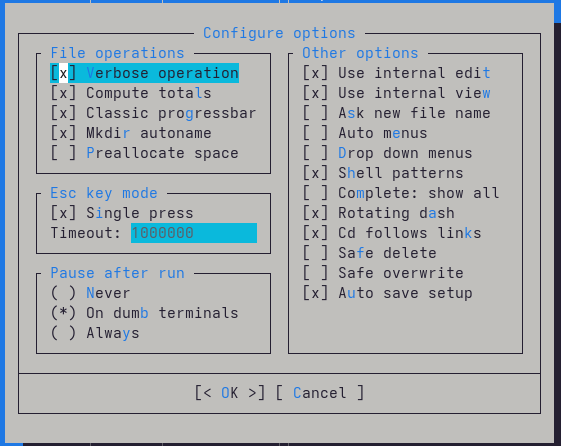
\includegraphics[width=0.7\linewidth,height=0.7\textheight]{image/19.png}

}

\caption{Конфигурация}

\end{figure}%
\end{frame}

\begin{frame}{Работа с Midnight Commander}
\phantomsection\label{ux440ux430ux431ux43eux442ux430-ux441-midnight-commander-19}
\begin{figure}

{\centering 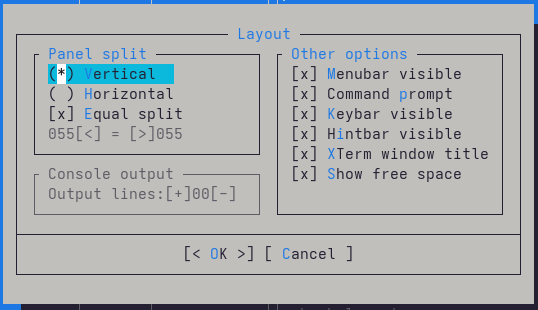
\includegraphics[width=0.7\linewidth,height=0.7\textheight]{image/20.png}

}

\caption{Внешний вид}

\end{figure}%
\end{frame}

\begin{frame}{Работа с Midnight Commander}
\phantomsection\label{ux440ux430ux431ux43eux442ux430-ux441-midnight-commander-20}
\begin{figure}

{\centering 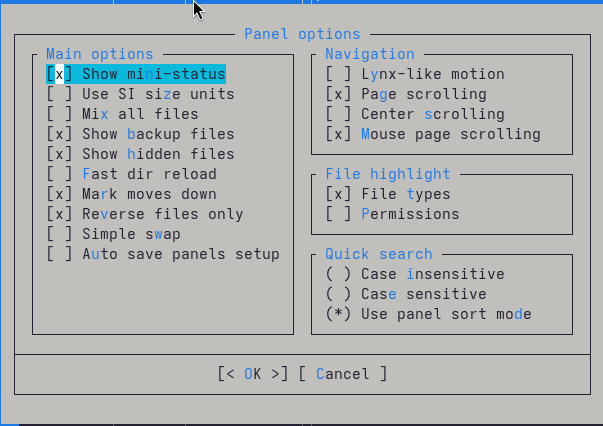
\includegraphics[width=0.7\linewidth,height=0.7\textheight]{image/21.png}

}

\caption{Настройки панелей}

\end{figure}%
\end{frame}

\begin{frame}{Работа с Midnight Commander}
\phantomsection\label{ux440ux430ux431ux43eux442ux430-ux441-midnight-commander-21}
\begin{figure}

{\centering 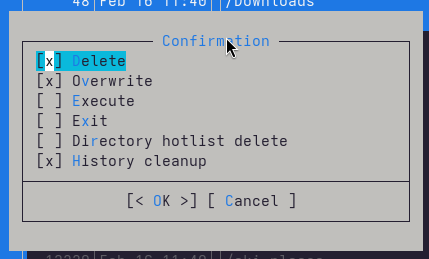
\includegraphics[width=0.7\linewidth,height=0.7\textheight]{image/22.png}

}

\caption{Подтверждение}

\end{figure}%
\end{frame}

\begin{frame}{Работа с Midnight Commander}
\phantomsection\label{ux440ux430ux431ux43eux442ux430-ux441-midnight-commander-22}
\begin{figure}

{\centering 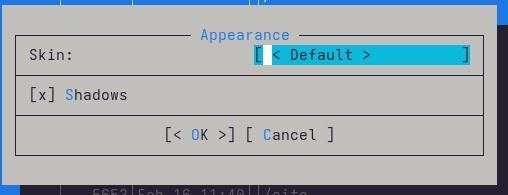
\includegraphics[width=0.7\linewidth,height=0.7\textheight]{image/23.png}

}

\caption{Оформление}

\end{figure}%
\end{frame}

\begin{frame}{Работа с Midnight Commander}
\phantomsection\label{ux440ux430ux431ux43eux442ux430-ux441-midnight-commander-23}
\begin{figure}

{\centering 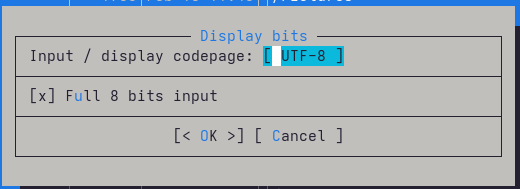
\includegraphics[width=0.7\linewidth,height=0.7\textheight]{image/24.png}

}

\caption{Кодировка символов}

\end{figure}%
\end{frame}

\begin{frame}{Работа с Midnight Commander}
\phantomsection\label{ux440ux430ux431ux43eux442ux430-ux441-midnight-commander-24}
\begin{figure}

{\centering 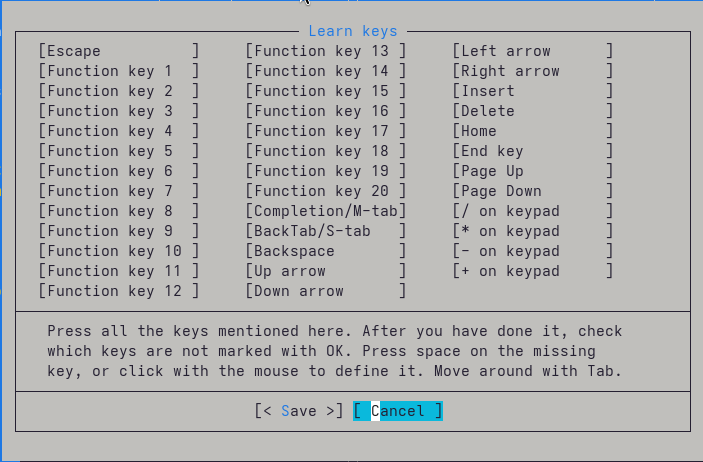
\includegraphics[width=0.7\linewidth,height=0.7\textheight]{image/25.png}

}

\caption{Распознавание клавиш}

\end{figure}%
\end{frame}

\begin{frame}{Работа с редактором Midnight Commander}
\phantomsection\label{ux440ux430ux431ux43eux442ux430-ux441-ux440ux435ux434ux430ux43aux442ux43eux440ux43eux43c-midnight-commander}
\begin{figure}

{\centering 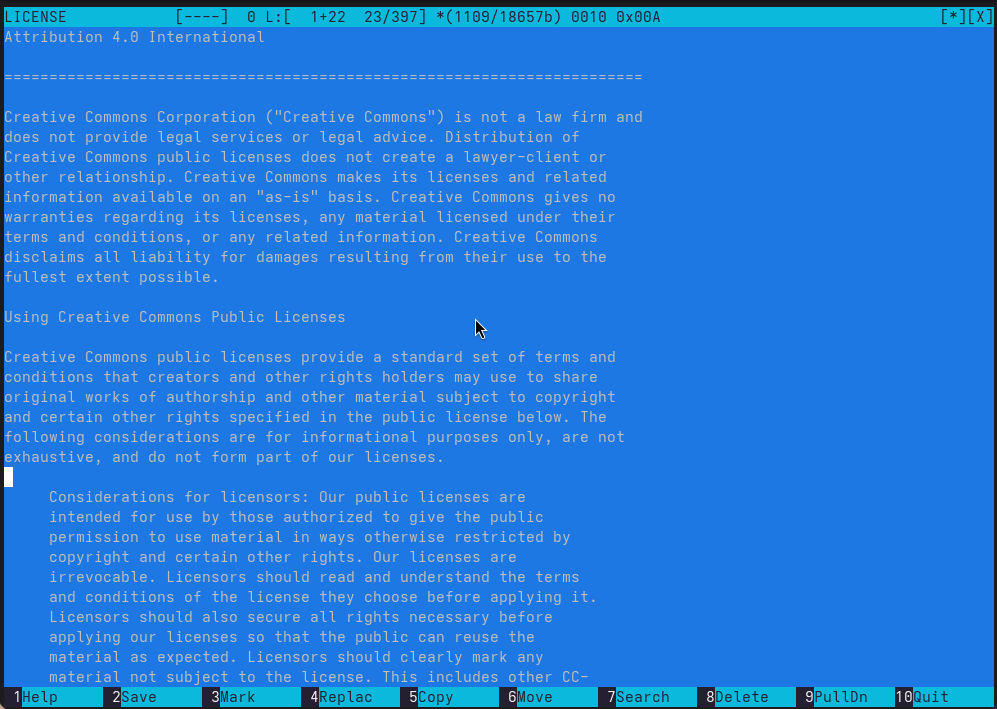
\includegraphics[width=0.7\linewidth,height=0.7\textheight]{image/26.png}

}

\caption{Файл с текстом}

\end{figure}%
\end{frame}

\begin{frame}{Работа с редактором Midnight Commander}
\phantomsection\label{ux440ux430ux431ux43eux442ux430-ux441-ux440ux435ux434ux430ux43aux442ux43eux440ux43eux43c-midnight-commander-1}
\begin{figure}

{\centering 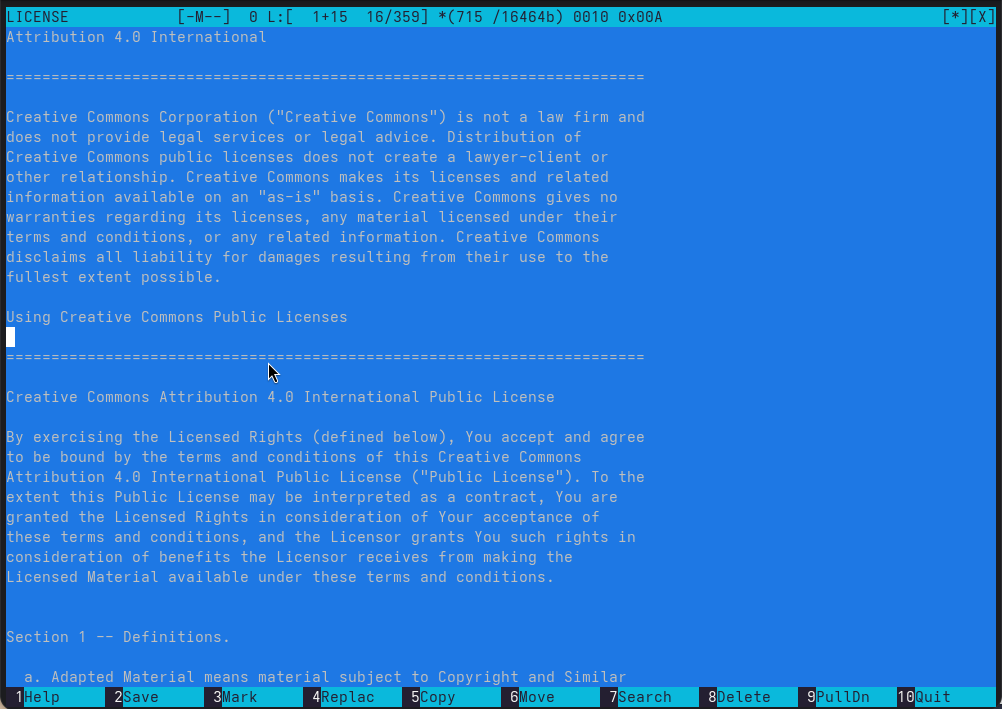
\includegraphics[width=0.7\linewidth,height=0.7\textheight]{image/27.png}

}

\caption{Файл с текстом}

\end{figure}%
\end{frame}

\begin{frame}{Работа с редактором Midnight Commander}
\phantomsection\label{ux440ux430ux431ux43eux442ux430-ux441-ux440ux435ux434ux430ux43aux442ux43eux440ux43eux43c-midnight-commander-2}
\begin{figure}

{\centering 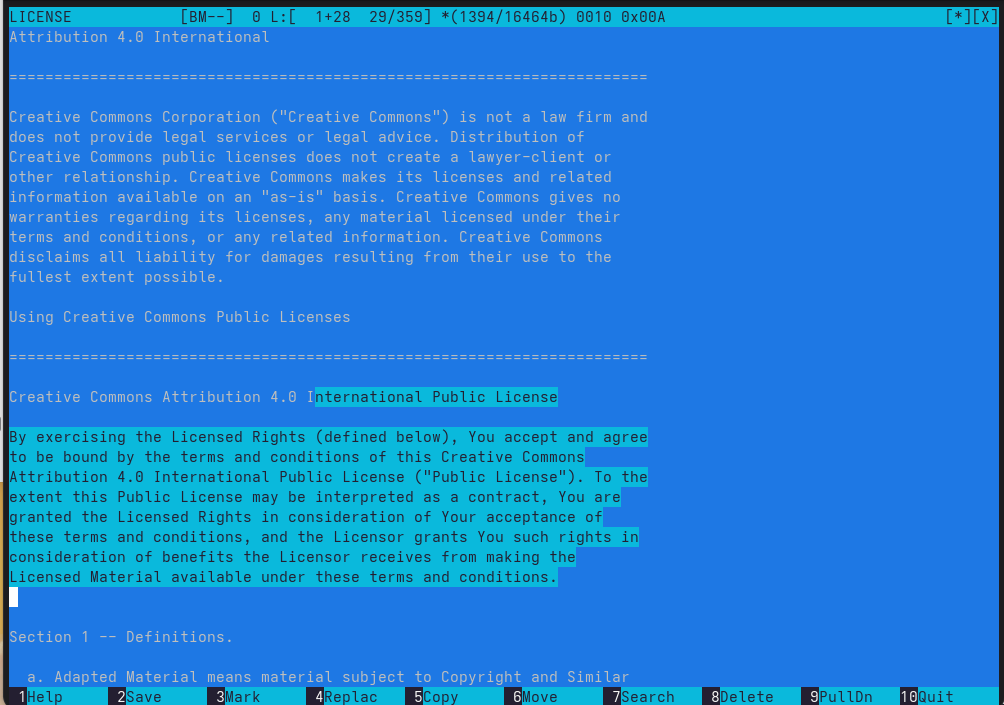
\includegraphics[width=0.7\linewidth,height=0.7\textheight]{image/28.png}

}

\caption{Копирование фрагмента}

\end{figure}%
\end{frame}

\begin{frame}{Работа с редактором Midnight Commander}
\phantomsection\label{ux440ux430ux431ux43eux442ux430-ux441-ux440ux435ux434ux430ux43aux442ux43eux440ux43eux43c-midnight-commander-3}
\begin{figure}

{\centering 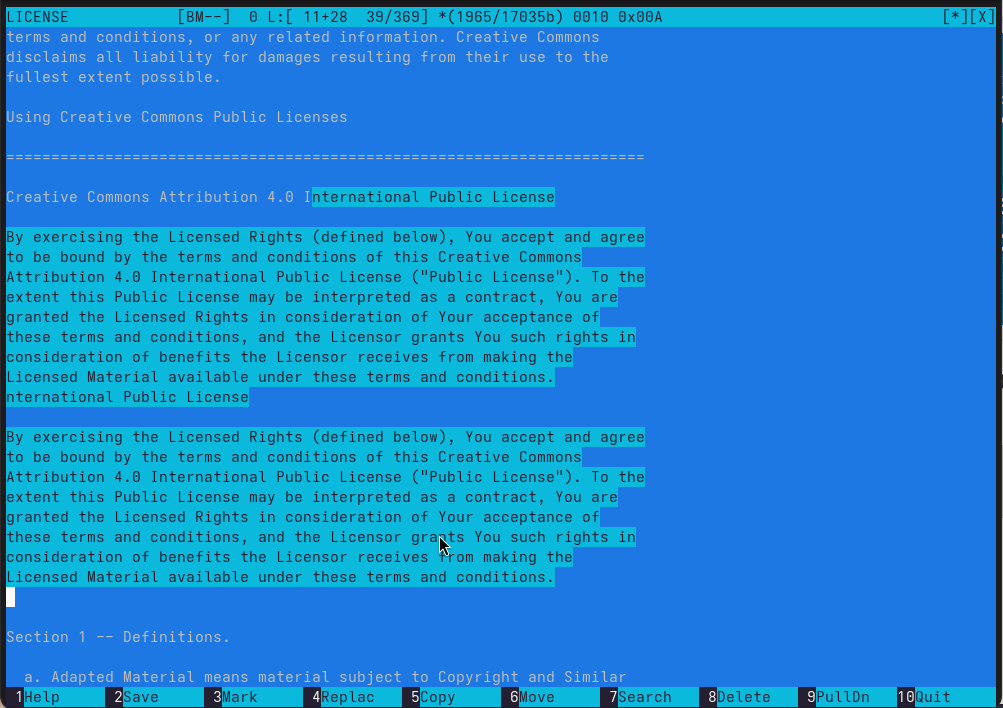
\includegraphics[width=0.7\linewidth,height=0.7\textheight]{image/29.png}

}

\caption{Сохранение}

\end{figure}%
\end{frame}

\begin{frame}{Работа с редактором Midnight Commander}
\phantomsection\label{ux440ux430ux431ux43eux442ux430-ux441-ux440ux435ux434ux430ux43aux442ux43eux440ux43eux43c-midnight-commander-4}
\begin{figure}

{\centering 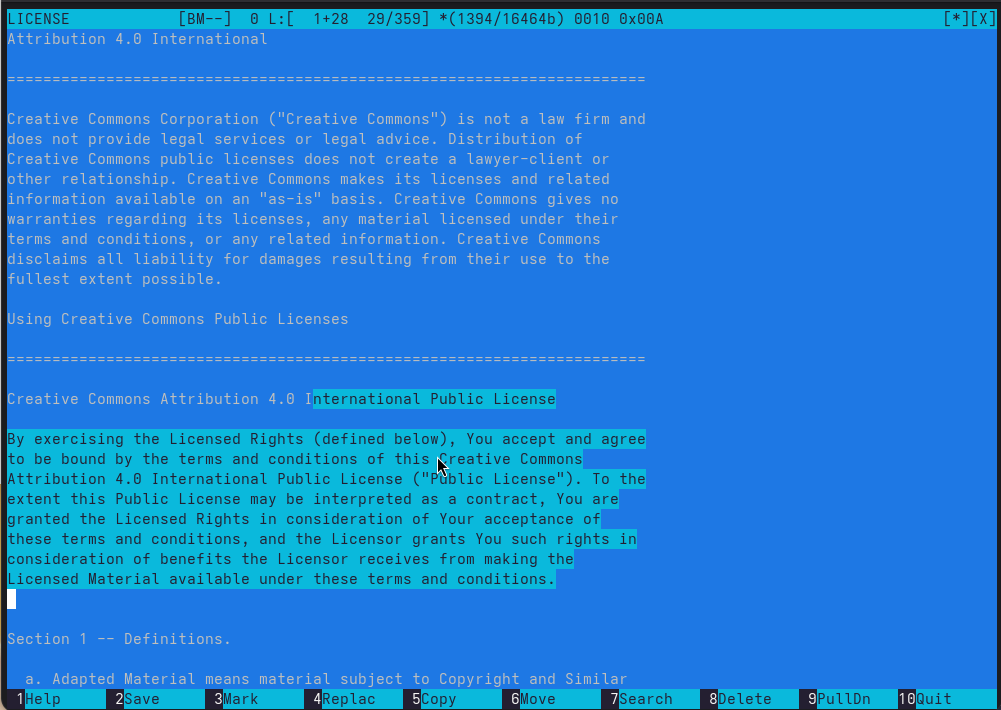
\includegraphics[width=0.7\linewidth,height=0.7\textheight]{image/30.png}

}

\caption{Отмена}

\end{figure}%
\end{frame}

\begin{frame}{Работа с редактором Midnight Commander}
\phantomsection\label{ux440ux430ux431ux43eux442ux430-ux441-ux440ux435ux434ux430ux43aux442ux43eux440ux43eux43c-midnight-commander-5}
\begin{figure}

{\centering 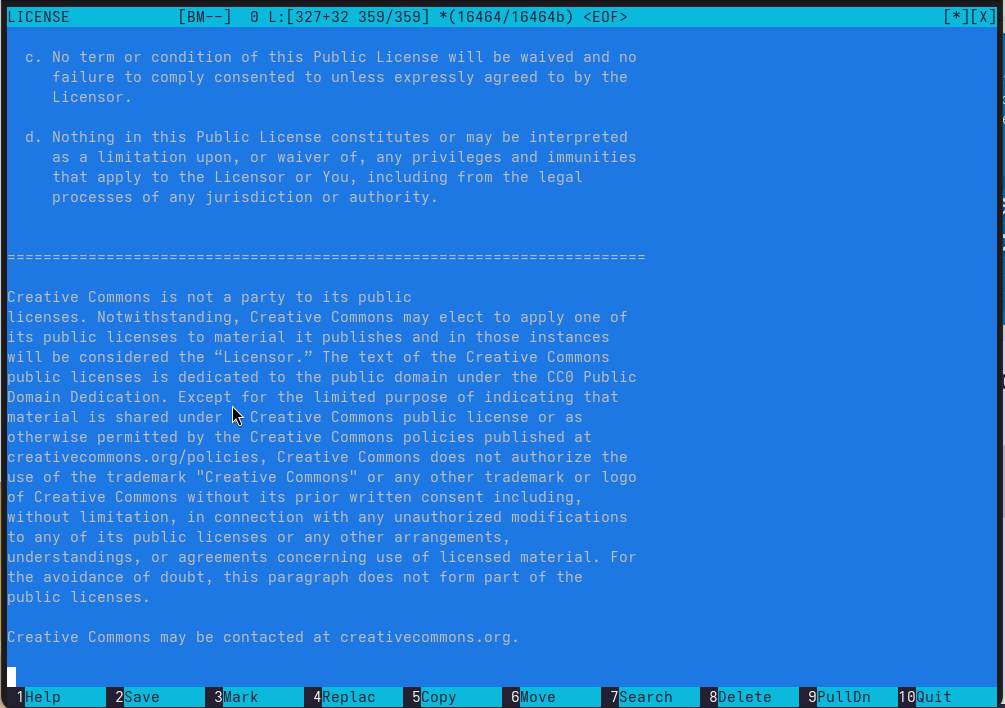
\includegraphics[width=0.7\linewidth,height=0.7\textheight]{image/31.png}

}

\caption{Переход в конец файла}

\end{figure}%
\end{frame}

\begin{frame}{Работа с редактором Midnight Commander}
\phantomsection\label{ux440ux430ux431ux43eux442ux430-ux441-ux440ux435ux434ux430ux43aux442ux43eux440ux43eux43c-midnight-commander-6}
\begin{figure}

{\centering 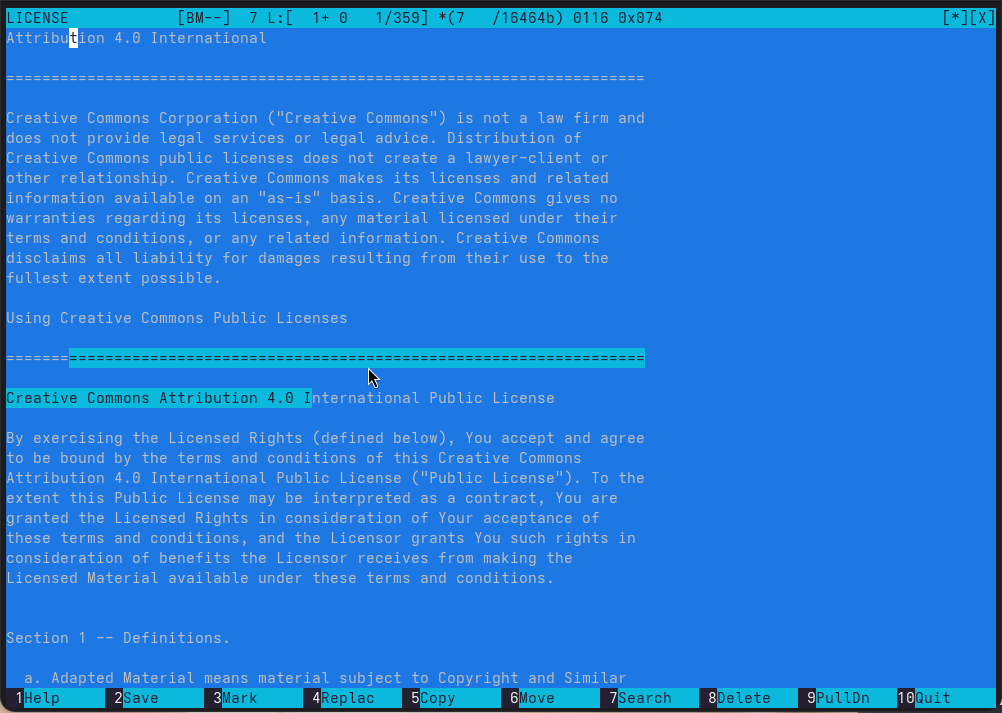
\includegraphics[width=0.7\linewidth,height=0.7\textheight]{image/32.png}

}

\caption{Переход в начало файла}

\end{figure}%
\end{frame}

\begin{frame}{Работа с редактором Midnight Commander}
\phantomsection\label{ux440ux430ux431ux43eux442ux430-ux441-ux440ux435ux434ux430ux43aux442ux43eux440ux43eux43c-midnight-commander-7}
\begin{figure}

{\centering 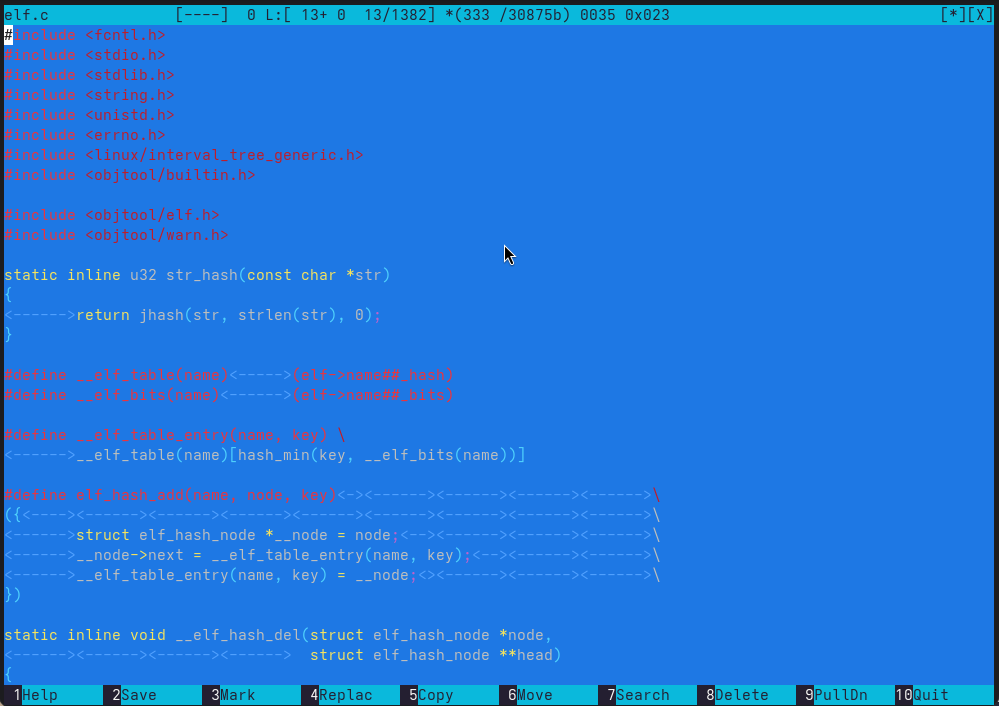
\includegraphics[width=0.7\linewidth,height=0.7\textheight]{image/33.png}

}

\caption{Файл с программой}

\end{figure}%
\end{frame}

\begin{frame}{Работа с редактором Midnight Commander}
\phantomsection\label{ux440ux430ux431ux43eux442ux430-ux441-ux440ux435ux434ux430ux43aux442ux43eux440ux43eux43c-midnight-commander-8}
\begin{figure}

{\centering 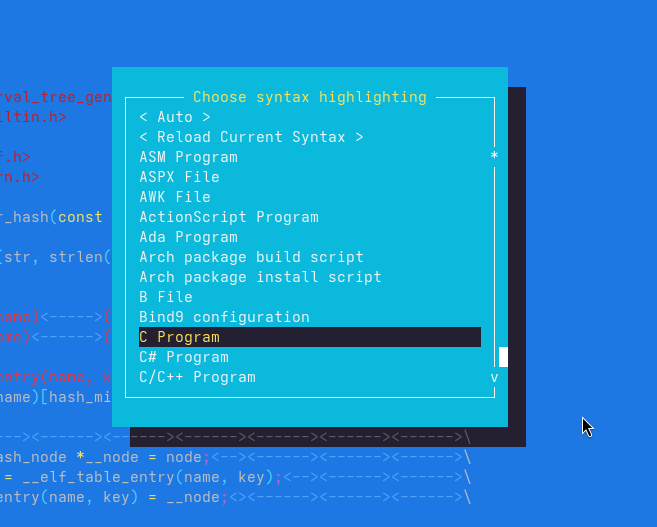
\includegraphics[width=0.7\linewidth,height=0.7\textheight]{image/34.png}

}

\caption{Цветовыделение синтаксиса}

\end{figure}%
\end{frame}

\section{Выводы по проделанной
работе}\label{ux432ux44bux432ux43eux434ux44b-ux43fux43e-ux43fux440ux43eux434ux435ux43bux430ux43dux43dux43eux439-ux440ux430ux431ux43eux442ux435}

\begin{frame}{Вывод}
\phantomsection\label{ux432ux44bux432ux43eux434}
В данной работе мы ознакомились с инструментами поиска файлов и
фильтрации текстовых данных. А также приобрели практические навыки по
управлению процессами.
\end{frame}




\end{document}
